% !TEX TS-program = xelatex
% !TEX encoding = UTF-8 Unicode
% !Mode:: "TeX:UTF-8"

\documentclass{resume}
\usepackage{graphicx}
\usepackage{tabu}
\usepackage{multirow}
\usepackage{progressbar}
\usepackage{zh_CN-Adobefonts_external} % Simplified Chinese Support using external fonts (./fonts/zh_CN-Adobe/)
% \usepackage{NotoSansSC_external}
% \usepackage{NotoSerifCJKsc_external}
% \usepackage{zh_CN-Adobefonts_internal} % Simplified Chinese Support using system fonts
\usepackage{linespacing_fix} % disable extra space before next section
\usepackage{cite}
\usepackage{fontspec}

\usepackage{hyperref}
\hypersetup{
    colorlinks=true,
    linkcolor=blue,
    filecolor=blue,      
    urlcolor=blue,
    citecolor=cyan,
}

\begin{document}
\pagenumbering{gobble} % suppress displaying page number

\Large{
  \begin{tabu}{ c l r }
   \multirow{4}{1in}{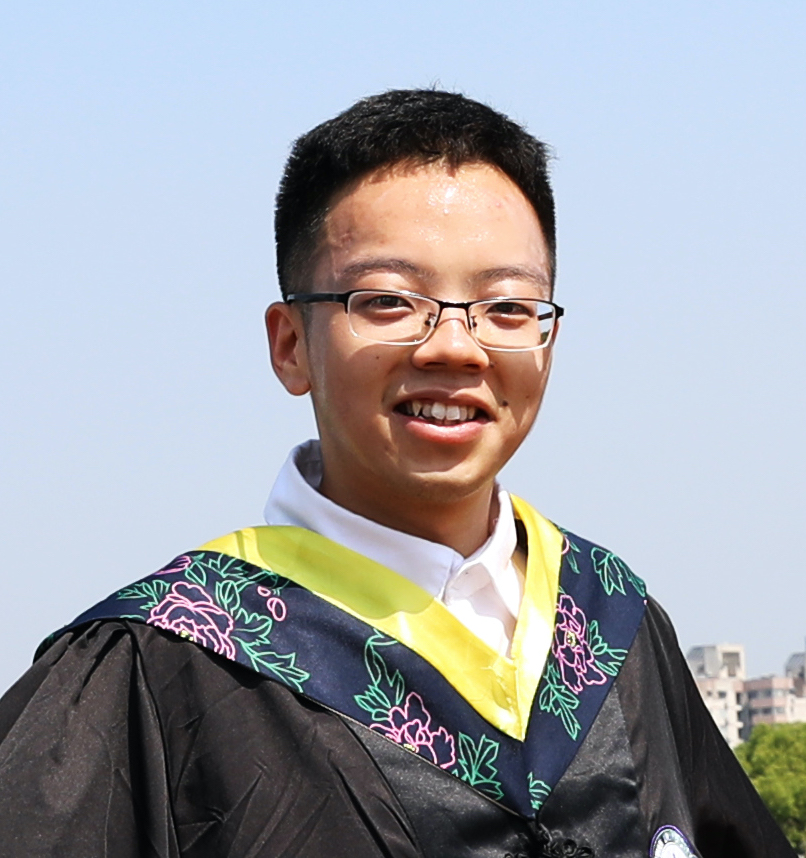
\includegraphics[width=0.95in]{img-me1.jpg}} & \scshape{张雪遥} &  \\
    & \email{xueyao\_98@foxmail.com} & \phone{(+86) 152-0390-0168} \\
    % & \phone{(+86) 152-0390-0168} &  \\
    & \faWechat{ xueyao\_98} & \github[github.com/RMSnow]{https://github.com/RMSnow} \\
    % & \github[github.com/RMSnow]{https://github.com/RMSnow} &
    & \faHome{\href{https://www.zhangxueyao.com}{~~zhangxueyao.com}}
    & \faMapMarker \small{北京市海淀区中关村街道科学院南路6号} 
  \end{tabu}
}

\section{教育背景}
\datedsubsection{\textbf{中国科学院计算技术研究所},计算机应用技术,学术型硕士\textit{(保研)}}{2019.09 -- 2022.06}
{\small 前瞻实验室,研究方向:大规模社交媒体数据挖掘,导师:曹娟研究员;GPA:3.79 / 4.00.}

\datedsubsection{\textbf{武汉大学},软件工程,学士}{2015.09 -- 2019.06}
{\small GPA:3.84 / 4.00,专业排名:4 / 246,英语六级:522.}


\section{研究经历}
\textbf{\large \framebox[1.2\width]{音乐生成}}
\datedsubsection{\textit{\textbf{Structure-Enhanced Pop Music Generation via Harmony-Aware Learning}}}{2021.07 -- 至今}
{\small \role{\textbf{Xueyao Zhang}, Jinchao Zhang, Yao Qiu, Li Wang, Jie Zhou}{投稿中;第一作者}
}
\small
\begin{itemize}
  \item \textit{研究任务} \quad .
  \item \textit{论文亮点} \quad .
  \item \textit{论文贡献} \quad .
\end{itemize}

\textbf{\\ \large \framebox[1.2\width]{虚假新闻检测}}

\datedsubsection{\textit{\textbf{Mining Dual Emotion for Fake News Detection} (Long Paper)}}{2020.04 -- 2021.04}
{\small \role{\textbf{Xueyao Zhang}, Juan Cao, Xirong Li, Qiang Sheng, Lei Zhong, Kai Shu.}{发表于\textit{WWW'2021};第一作者}
}
\small
\begin{itemize}
  \item \textit{研究任务} \quad 虚假新闻检测(Fake News Detection):给定一条社交媒体的新闻(如微博、Tweet),判定其真实性(Fake / Real).
  \item \textit{论文亮点} \quad 虚假新闻在写作风格上常常拥有强烈的情感(发布者情感),且常常能够引发公众的特定情绪(社交情感)。本篇论文基于此提出了双重情感特征(Dual Emotion),用来增强现有模型的检测能力.
  \item \textit{论文贡献} \quad 论文在一个Twitter数据集、两个微博数据集(其中一个为本论文首次公布)上,均证实了双重情感特征的有效性。论文相关资源的公开地址:\href{https://www.zhangxueyao.com/data/www2021-dual-emotion-paper.pdf}{[PDF]} \href{https://github.com/RMSnow/WWW2021}{[Code]} \href{https://www.zhangxueyao.com/assets/www2021-dual-emotion-slides.pdf}{[Slides]} \href{https://www.zhangxueyao.com/assets/www2021-dual-emotion-video.mp4}{[Video]} \href{https://www.bilibili.com/video/BV13o4y1m7c3}{[Chinese Video]}.
\end{itemize}

\datedsubsection{\textit{\textbf{Integrating Pattern- and Fact-based Fake News Detection via Model Preference Learning} (Long Paper)}}{2021.02 -- 2021.11}
{\small \role{Qiang Sheng*, \textbf{Xueyao Zhang}*, Juan Cao, Lei Zhong. (*: Equal Contribution)}{发表于\textit{CIKM'2021};共同一作}
}
\small
\begin{itemize}
  \item \textit{研究任务} \quad 虚假新闻检测(Fake News Detection):给定一条社交媒体的新闻(如微博、Tweet),判定其真实性(Fake / Real).
  \item \textit{论文亮点} \quad 基于模式的和基于事实的虚假新闻模型,这两者对于待查新闻中的.
  \item \textit{论文贡献} \quad .
\end{itemize}

\datedsubsection{\textit{\textbf{Article Reranking by Memory-enhanced Key Sentence Matching for Detecting Previously Fact-checked Claims} (Long Paper)}}{2020.09 -- 2021.08}
{\small \role{Qiang Sheng, Juan Cao, \textbf{Xueyao Zhang}, Xirong Li, Lei Zhong.}{发表于\textit{ACL'2021};学生第二作者}}
\small
\begin{itemize}
  \item \textit{研究任务} \quad 检测“旧谣新传”(Detecting Previouly Fact-checked Claims):给定一条谣言,在已有的辟谣库中,检索其相关的辟谣文档。该任务可以为谣言的判别提供“事实性证据”.
  % \item \textit{技术路线} \quad 现有的检索流程常分为两个阶段:(1)基于BM25等传统检索模型的粗排序;(2)基于BERT等深度模型的重排序。本文着力于设计第二阶段的重排序模型.
  \item \textit{论文亮点} \quad (1)基于挑选关键句来进行相关文档检索,因此模型具有句子级别的可解释性;(2)除了利用词汇重合信息、语义相似信息进行检索之外,本文还借助Memory机制,捕捉辟谣文章中常见的写作模式特征;(3)构建了该研究任务的第一个中文数据集.
  \item \textit{个人贡献} \quad 进行Coding,完成大部分实验。论文相关资源的公开地址:\href{https://aclanthology.org/2021.acl-long.425.pdf}{[PDF]} \href{https://github.com/ICTMCG/MTM}{[Code]} \href{https://www.zhangxueyao.com/data/acl2021-MTM-poster.pdf}{[Poster]} \href{https://zhuanlan.zhihu.com/p/393615707}{[Chinese Blog]}.
\end{itemize}

\section{实习经历}
\datedsubsection{\textbf{腾讯 - WXG(微信事业群) - 模式识别中心}}{2021.04 -- 至今}
{\small \role{部门总监:周杰;直属领导:张金超.}{\textbf{音乐生成算法实习生}}
}
\small
\begin{itemize}
  % \item \textit{业务场景} \quad 为微信视频号中用户上传的视频自动配乐.
  \item 负责音乐生成算法的研发;提供音乐背景、乐理知识等支持,专业化地评估人工智能音乐.
  \item 举办了一次内部的音乐培训讲座:\href{https://www.zhangxueyao.com/data/wcpr-pop-music.pdf}{\underline{一首流行歌是如何创作?}}
\end{itemize}

\section{音乐能力}
\small
\begin{itemize}
  \item 掌握基础的乐理知识,熟悉常见的音乐风格.
  \item 熟悉流行音乐的键盘演奏,了解吉他演奏.
  \item 爱好流行演唱,曾获中国科学院大学校园歌手大赛季军;拥有合唱团演唱、领唱经历.
  \item 对计算音乐学、音乐生成、音乐理解等领域具有浓厚的兴趣. 
\end{itemize}

\section{编程技能}
\small
\begin{itemize}
  \item 编程语言:熟练使用Python,了解Java、C++.
  \item 深度学习框架:PyTorch、Keras.
\end{itemize}

\section{获奖情况}
\begin{itemize}
  \item 中国科学院大学校园歌手大赛季军(2020)
  \item 中国科学院大学计算机学院三好学生(2019;2020)
  \item 武汉大学优秀学士学位论文(2019)
  \item 武汉大学三好学生、优秀团员、优秀学生干部(2016;2017;2018)
  \item 本科生国家奖学金(2016)
  \item 全国高中生数学联赛一等奖(2014)
\end{itemize}

\end{document}
